\section{Tensor Field Visualisatio}
\subsection{Tensors}
\begin{quote}{H. Hagen:}
    Tensors are the language of mechanics.
\end{quote}
Tensors of \emph{order} (rank):
\begin{description}
\item[0]: Scalar
\item[1]: Vector
\item[2]: Matrix
\end{description}
Tensors can have "lower" and "upper" indices indicating different transformation rules for change of coordinates.

Tensor field visualisation almost always deals with \emph{$2^{nd}$ order tensors}. Eigenvectors and eigenvalues contain full information.

Separate visualisation methods for \emph{symmetric} and \emph{nonsymmetric} tensors. Visualisation methods for tensor fields include:
\begin{itemize}
    \item Tensor glyphs
    \item Tensor field lines, hyperstreamlines
    \item Tensor field topology
    \item Fiber bundle tracking.
\end{itemize}

\subsection{Tensor Glyps}
In 3D, tensors are $3\times 3$ matrices. The \emph{velocity gradient tensor} is non-symmetric:  $9$ degrees of freedom for the local change of the velocity vector. 

A \emph{glyph} developed by de Leeuw and van Wijk can visualise all these $9$ DOFs:
\begin{itemize}
    \item Tangential acceleration: Green "membrane"
    \item Orthogonal acceleration: Curvature of arrow
    \item Twist: Candy stripes
    \item Shear: Orange ellipse
    \item Convergence/divergence: White "parabolic reflector"
\end{itemize}

\paragraph{Symmetric 3D tensors}  Real eigenvalues, orthogonal eigenvectors. If \emph{positive definite} the data can be represented by \emph{ellipsoids}.

Three types of anisotropy:
    \begin{itemize}
        \item Linear anisotropy
        \item Planar anisotropy
        \item Isotropy (spherical)
    \end{itemize}
    
Anisotrpoy measure:
\begin{align*}
    c_1 &= {\lambda_1-\lambda_2 \over \lambda_1+\lambda_2+\lambda_3}\\
    c_p &= 2{\lambda_2-\lambda_3 \over \lambda_1+\lambda_2+\lambda_3}\\
    c_s &= 3{\lambda_3 \over \lambda_1+\lambda_2+\lambda_3}
\end{align*}

\begin{figure}[H]
\centering
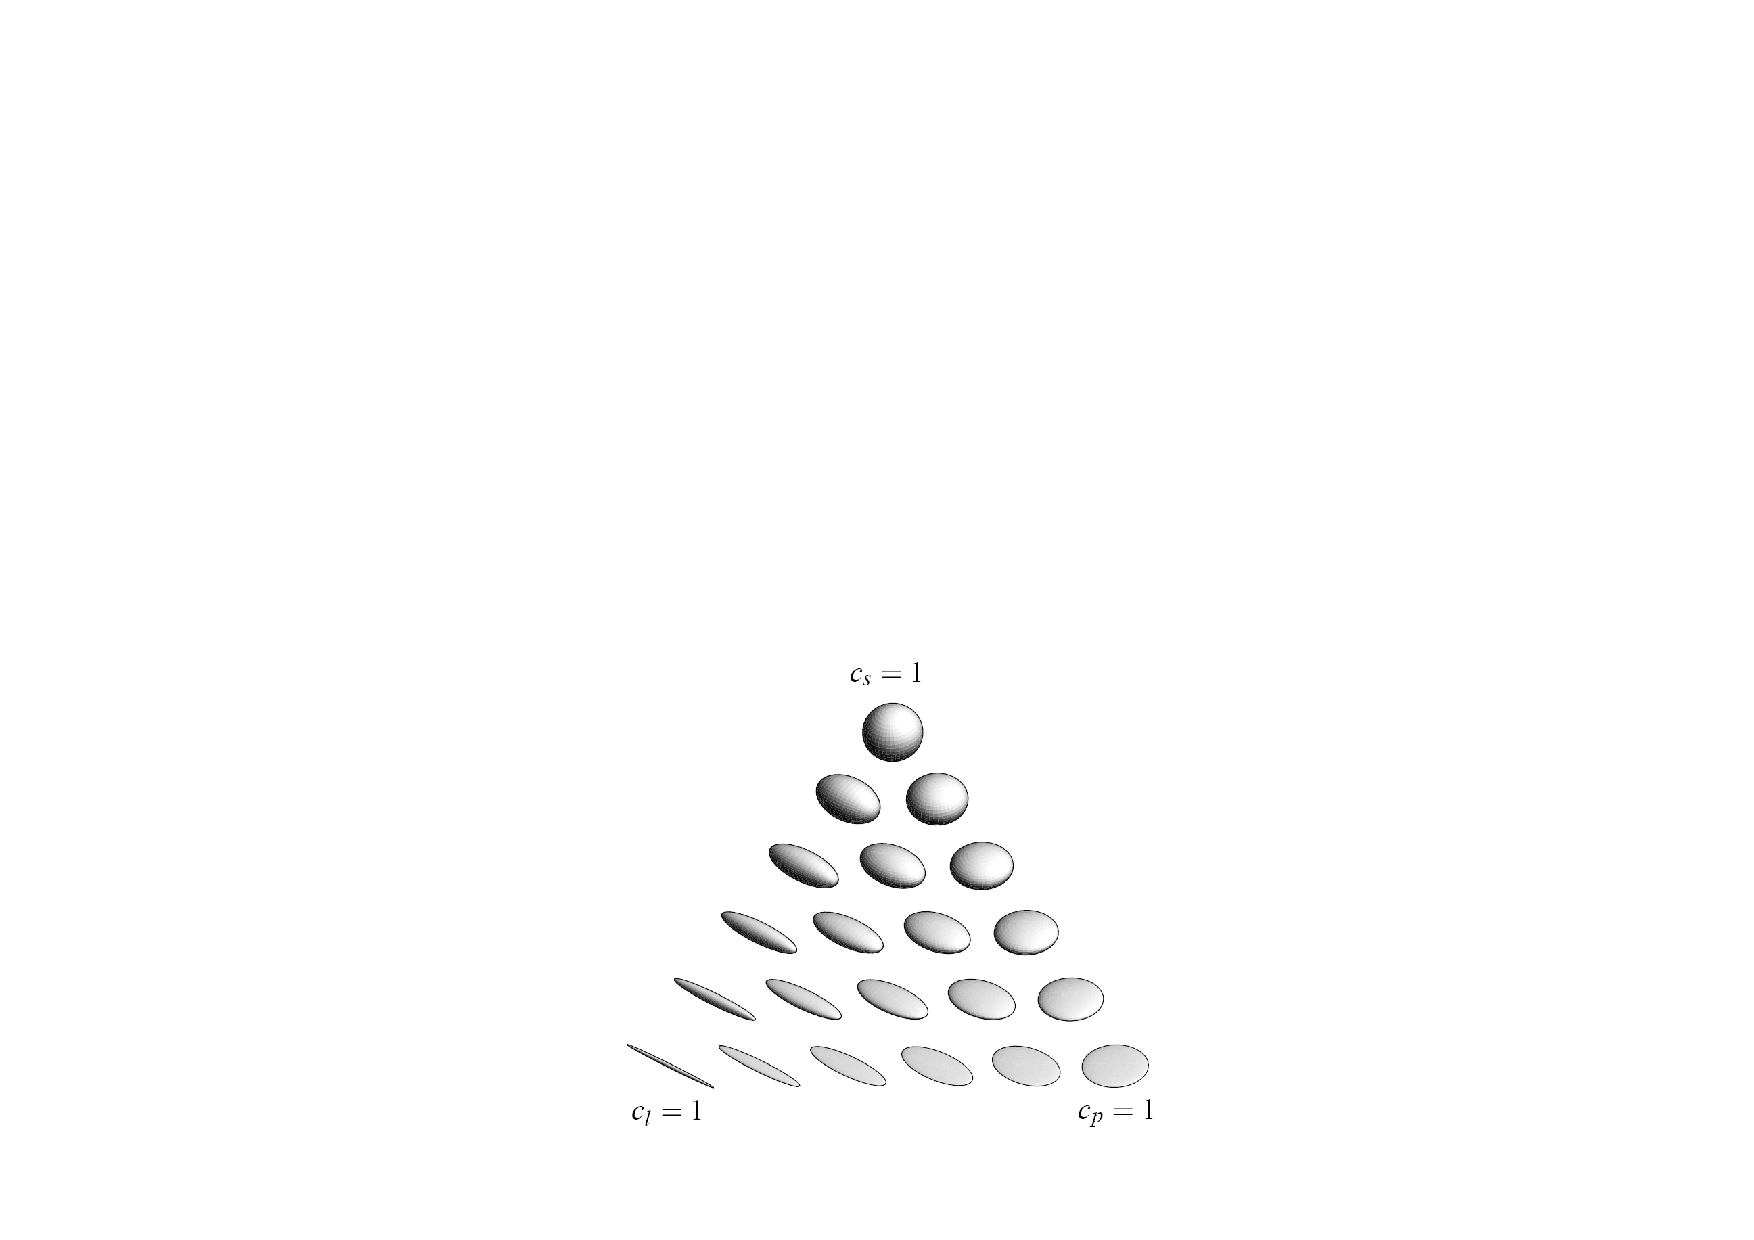
\includegraphics[width=0.4\textwidth]{img/10_3d_tensors}
\end{figure}

Problem of \emph{ellipsoid} glyphs:
The shape is poorly recognised in projected views.

Problem of \emph{cuboid} glyphs: Small differences in eigenvalues are overemphasised.

Problem of \emph{cylinder} glyphs: Discontinuity at $c_l = c_p$ and artificial orientation at $c_s =1$.

\paragraph{Superquardics} Combining advantegs.

Superquadrics with $z$ as primary axis:
\begin{align*}
    q_z (\theta,\phi) = \begin{pmatrix}
                             \cos^{\alpha} \theta \sin^{\beta}\phi\\
                             \sin^{\alpha} \theta \sin^{\beta}\phi\\
                             \cos^{\beta} \phi
                        \end{pmatrix}
\end{align*}
with $\cos^{\alpha}\theta$ used as shorthand for $|\cos\theta|^\alpha sgn(\cos\theta)$.
\paragraph{Superquadric Glyphs} (G. Kindlmann): Given $c_l$, $c_p$ and $c_s$.
\begin{itemize}
    \item Compute a base superquardic using a \emph{sharpness} value $\gamma$:
        \begin{align*}
            q(\theta, \phi) = 
                \begin{cases}
                     c_l \geq c_p: & q_z (\theta, \phi)  \text{ with $\alpha = (1-c_p)^\gamma$  and $\beta = (1-c_l)^\gamma$}\\
                     c_l < c_p:    & q_x (\theta, \phi)  \text{ with $\alpha = (1-c_l)^\gamma$  and $\beta = (1-c_p)^\gamma$}
                \end{cases}
        \end{align*}
    \item Rotate into eigenvector frame and scale with $\lambda_1$, $\lambda_2$ and $\lambda_3$.
\end{itemize}
\begin{figure}[H]
\centering
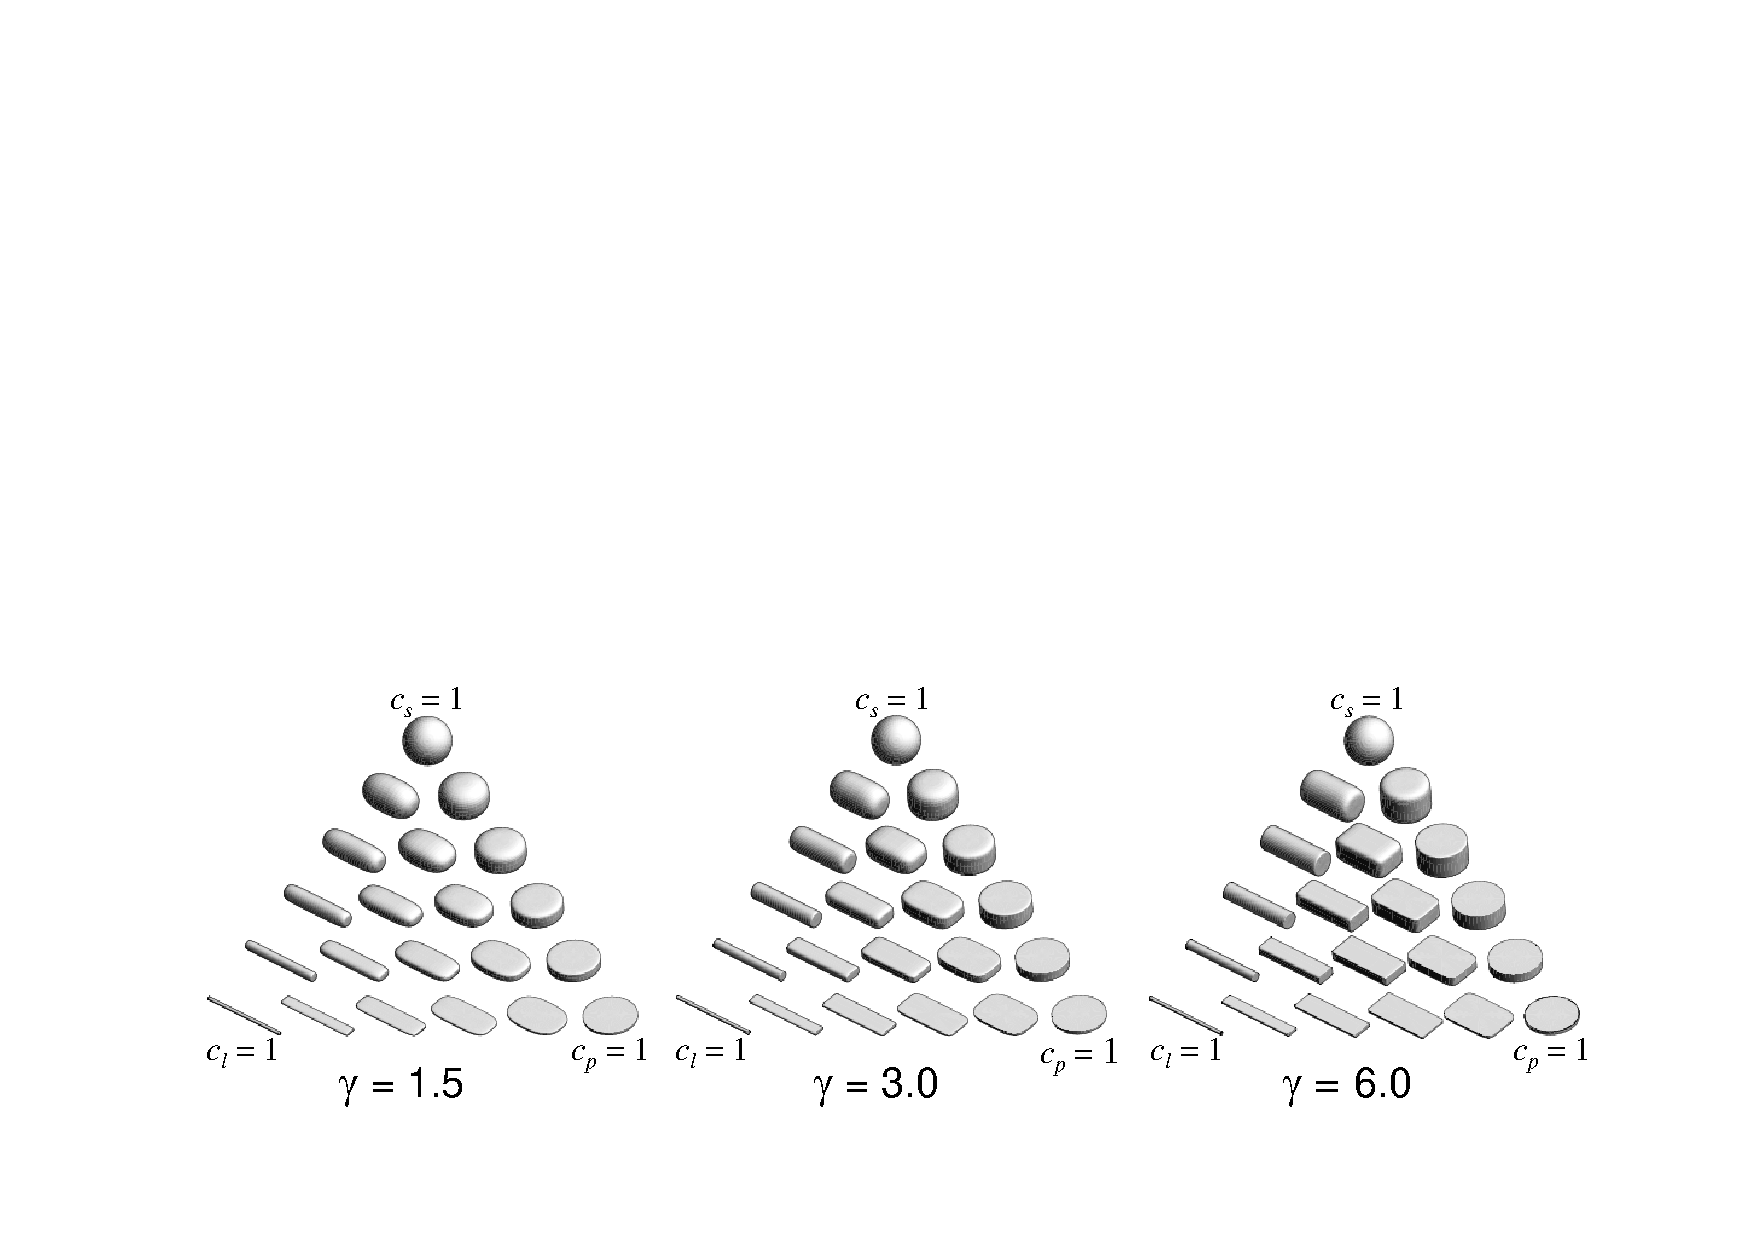
\includegraphics[width=0.8\textwidth]{img/10_superquadrics}
\end{figure}

\subsection{Tensor Field Lines}
Let $T(x)$ be a $2^{nd}$ order symmetric tensor field (real eigenvalues, orthogonal eigenvectors).

\paragraph{Tensor field line} Compute by integrating along one of the eigenvectors. Important: Eigenvector fields are \emph{not} vector fields:
\begin{itemize}
    \item Eigenvectors have \emph{no magnitude} and \emph{no orientation} 
    \item The \emph{choice} of the eigenvector (minor, major) can be made consistently only as long as all eigenvalues are all different.
    \item Tensor field lines can \emph{intersect} (only) at points where two or more eigenvalues are equal, so-called \emph{degenerate points}.b
\end{itemize}

Tensor field lines can be rendered as \emph{hyperstreamlines}: Tubes with an elliptic cross section and a radius proportional to the $2^{nd}$ and $3^{rd}$ eigenvalue.

Based on tensor field lines, a \emph{tensor field topology} can be defined in analogy to the the vector field topology.

Degenerate points play the role of critical points. At degenerate points infinitely many directions (of eigenvectors) exist. 

For simplicity we only study the \emph{2D} case. A $2\times 2$ tensor at a degenerate point has (in the given coordinate frame!) the form
\begin{align*}
 T =
     \begin{pmatrix}
         \lambda & 0\\
         0 &\lambda
     \end{pmatrix} = \lambda 1.
\end{align*}
Hence, degenerate points are found by solving the equations
\begin{align*}
    T_{11}(x) - T_{22}(x) &= 0\\
    T_{12}(x) &= 0
\end{align*}

\paragraph{Types of degenerate points} illustrated with linear tensor fields:
\begin{figure}[H]
    \centering
    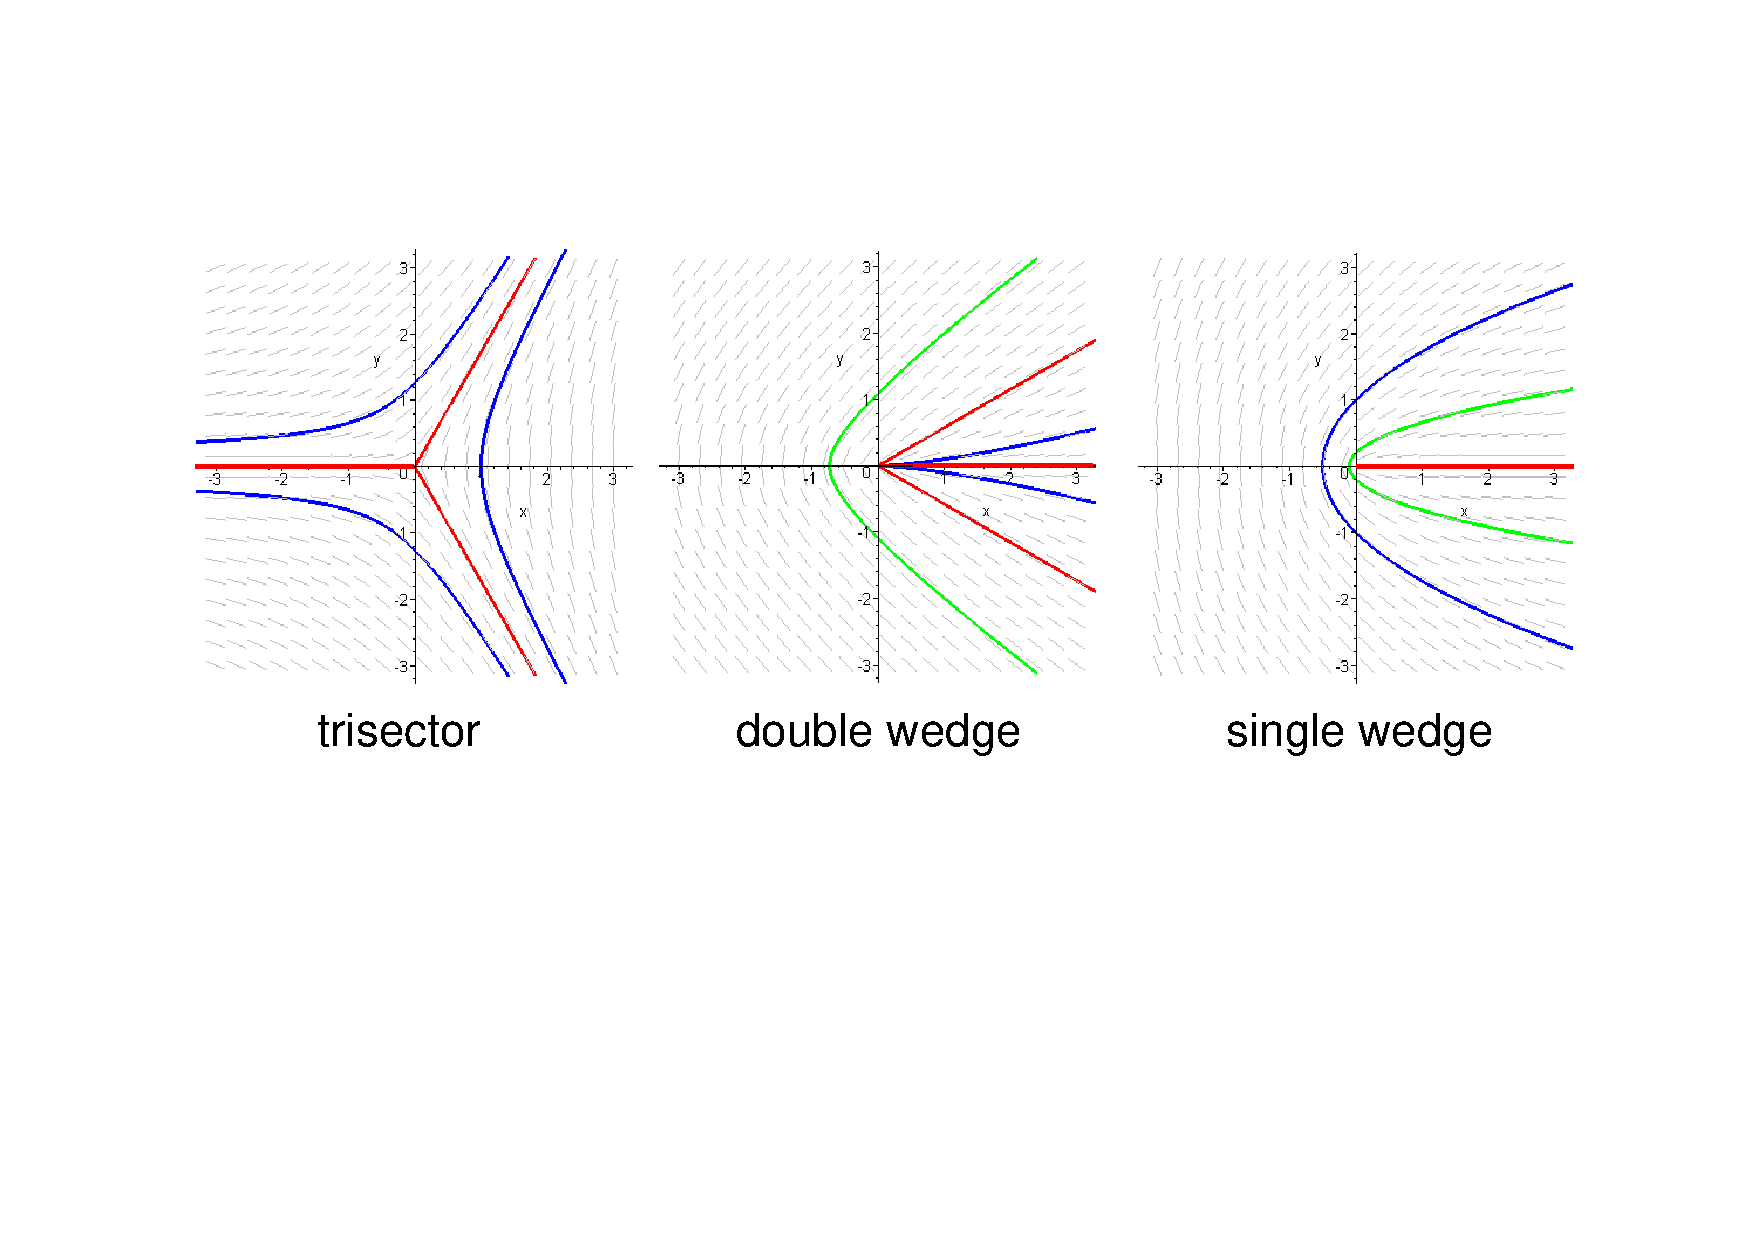
\includegraphics[width=0.8\textwidth]{img/10_tensor_field_degenerate_points}
\end{figure}

\paragraph{Separatrices} are tensor field lines converging to the degenerate point with a radial tangent.  

They are straight lines in the special case of a linear tensor field.

\paragraph{Double Wedges} Have one "hidden separatrix" and two other separatrices which actually separate regions of different field line behaviour. 

\paragraph{Single Wedges} Have just one separatrix.

Saddles, nodes and foci can exist as non-elementary (higher-order) degenerate points. They are created by merging trisectors or wedges. They are not structurally stable and break up in their elements if perturbed. 
\begin{figure}[H]
\centering
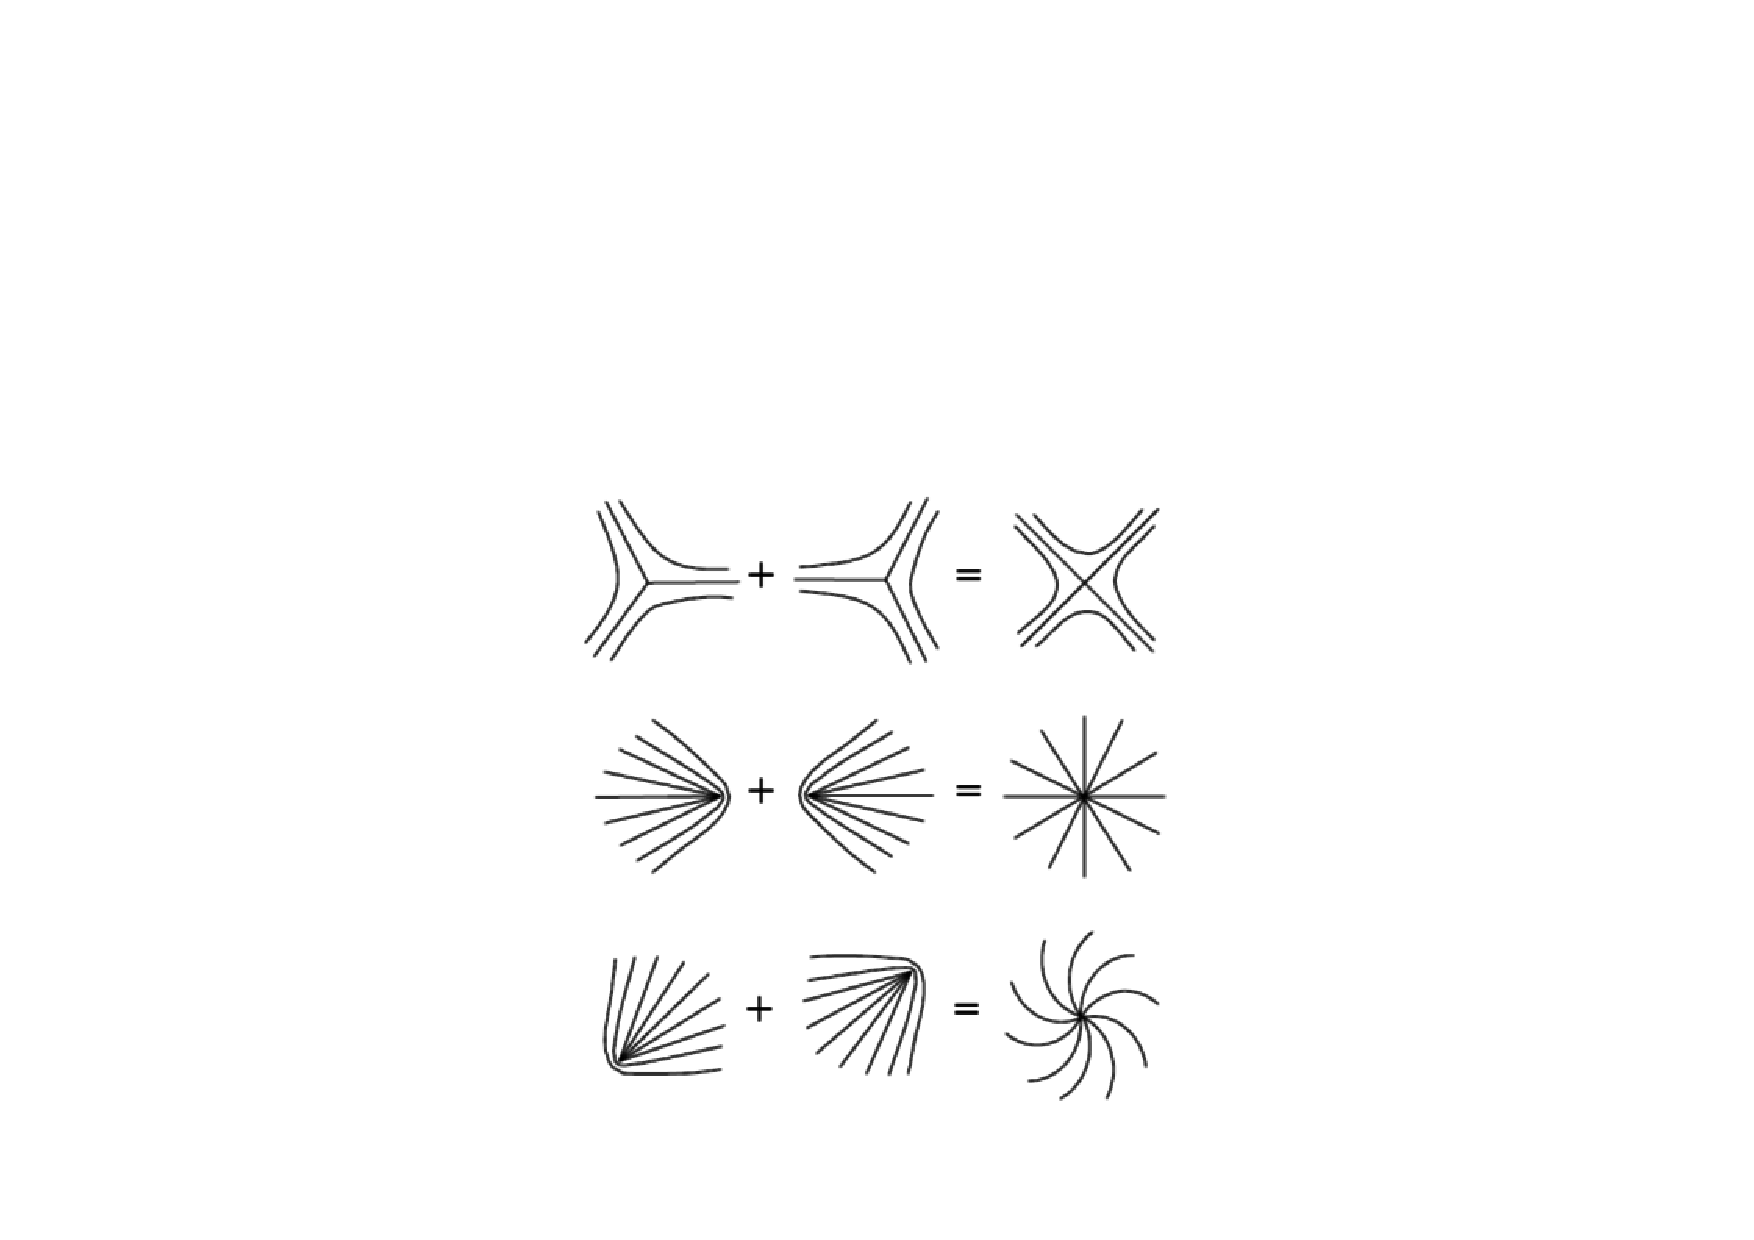
\includegraphics[width=0.4\textwidth]{img/10_merging_tensor_fields}
\end{figure}

\paragraph{Topological Skeleton} The \emph{topological skeleton} is defined as the set of separatrices of trisector points.

\subsection{Diffusion Tensor Fiber Bundle Tracking}
DTI is a newer magnetic resonance imaging (MRI) technique. DTI produces a tensor field of the anisotropy of the brain's white matter.

Most important application: \emph{Tracking fiber bundles}.

Interpretation of anisotropy types:
\begin{itemize}
\item Isotropy: No white matter
\item Linear anisotropy: Direction of the fiber bundle
\item Planar anisotrpoy: Can have different meanings!
\end{itemize}

Fiber bundle tracking $\neq$ tensor field line integration because bundles may \emph{cross} each other. 

\paragraph{Method 1} \emph{Best neighbour} algorithm (Poupon), based on the idea of restricting the curvature:
\begin{itemize}
    \item At each voxel compute the eigenvector of the dominant eigenvalue. 
    
     Get a "direction map.
    \item At each voxel $M$ find the "best neighbour voxel" $P$ according to angle dcriterion. Get a "tracking map".
    \item Connect voxels (within a "white matter mask") with its best neighbour. 
\end{itemize}

\paragraph{Method 2} Apply \emph{moving least squares} filter which favors the current direction of the fiber bundle (Zhukov and Barr).
\begin{figure}[H]
    \centering
    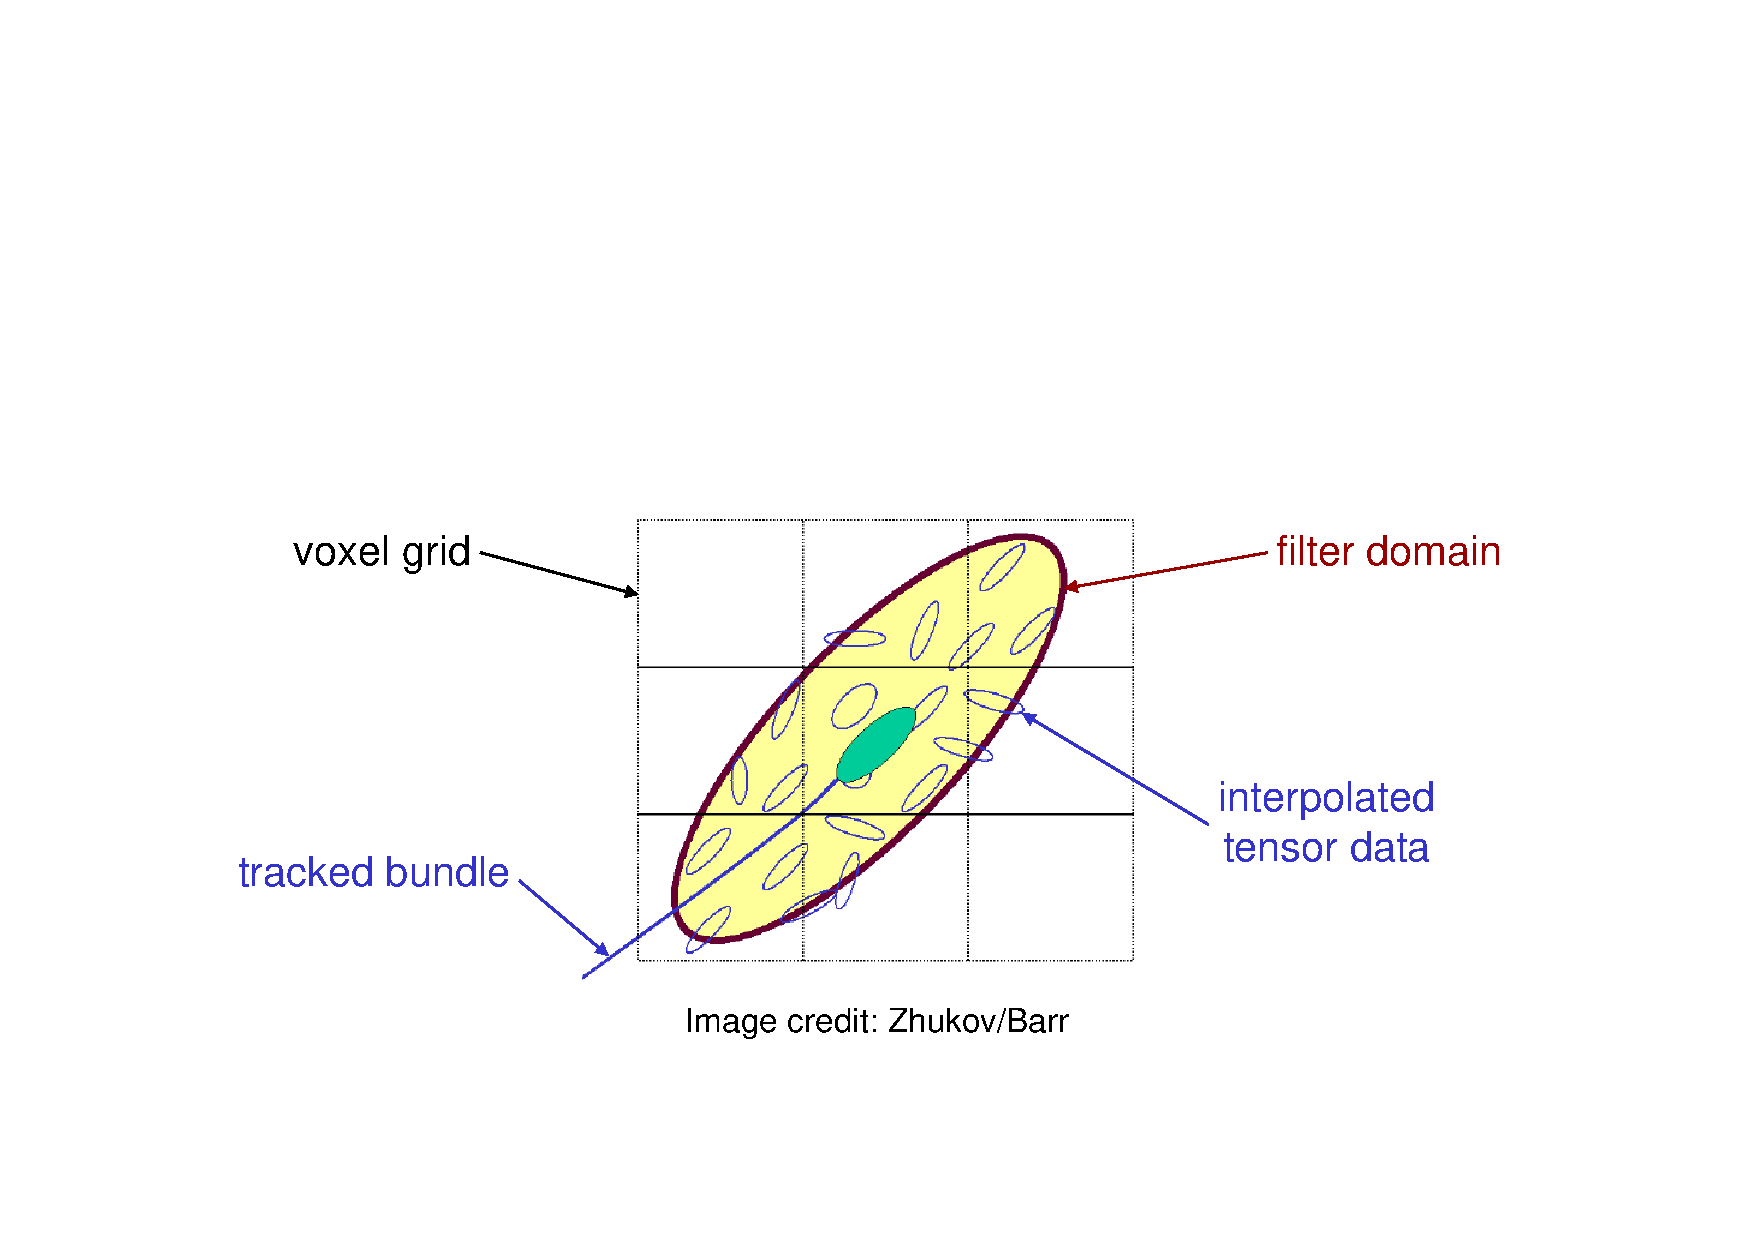
\includegraphics[width=0.6\textwidth]{img/10_dti_mls}
\end{figure}

\paragraph{Method 3} \emph{Tensor deflection} (TEND, Lazar et al.) 

Idea: If $v$ is the incoming bundle direction use $Tv$ as the direction of the next step.

Reasoning:
\begin{itemize}
    \item $Tv$ bends the curve towards the dominant eigenvector.
    \item $Tv$ has the unchanged direction of $v$ if $v$ is 
        \begin{itemize}
            \item An eigenvector of $T$,
            \item Or a vector within the eigenvector plane if the two dominant eigenvalues are equal (rotationally symmetric $T$.
        \end{itemize}
\end{itemize}


\subsubsection{Algorithmic Steps}
Clustering of fibers: The goal is to identify nerve tracts.

\begin{enumerate}
    \item \emph{Clustering} based on geometric attributes (centroid, variance, curvature).
    
    Possible method: $n$-dimensional mass-spring model.
    \item \emph{Center line}: Take sets of "corresponding vertices" of each bundle and average them.
    
    \item \emph{Wrapping surface}: Compute the convex hull in orthogonal slices using Graham's scan algorithm.
\end{enumerate}

































